\subsection{Utledning av bølgeligningen}
\subsubsection{Forhåndsbetingelser}
For å finne frem til bølgeligningen må en se på hvordan systemet en skal bruke likningen i ser ut.
På en gitar er lengden på strengen justerbar, men en endrer tonen ved å stramme eller slakke
på gitarstrengen.

En gitarstreng kan modelleres som en tråd som er spent mellom to punkter, der den er fiksert på plass.
I normaltilstand ligger strengen spent i en rett linje mellom punktene, frem til den blir plukket. Da
har den blitt forstyrret, og strengen begynner å vibrere. Problemet er da å finne en \(u(x,t)\) som modellerer
defleksjonen til strengen. Hvis strengen har lengde \(l\), massetetthet \(\rho\) og blir sluppet løs ved \(t=0\),
vil formelen finne defleksjonen til strengen for hvilken som helst \(x\) når \(t>0\).

For å løse likningen trengs det noen forhåndsbetingelser.

\begin{enumerate}
  \item Gravitasjon er neglisjerbar i forhold til strengspenningen.
  \item Alle defleksjoner er små og skjer i samme plan.
  \item Massen per lengde er konstant over hele strengen, slik at spenningen er den samme
  gjennom hele strengen.
\end{enumerate}

\subsubsection{Utledning}

\begin{figure}[h]
\centering
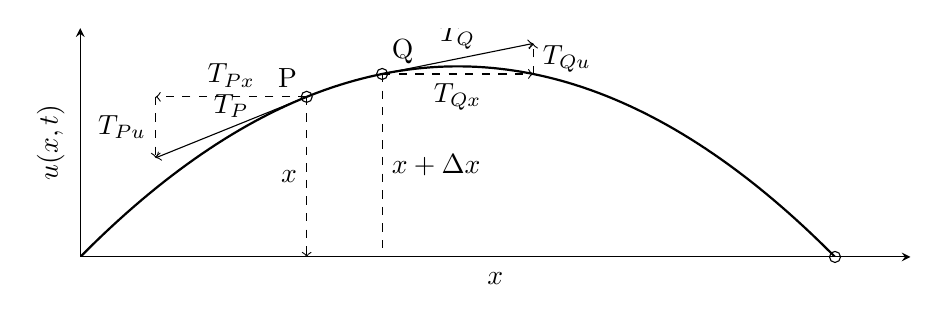
\begin{tikzpicture}
\begin{axis}[
  width=\textwidth,
  height=0.37\textwidth,
  axis lines=left,
  xlabel={$x$},
  ylabel={$u(x,t)$},
  xmin=0, xmax=1.1,
  ymin=0, ymax=0.6,
  xtick=\empty,
  ytick=\empty
]
  % punkter
  \coordinate (Ppoint)  at (axis cs:0.3,0.42);
  \coordinate (Pupoint) at (axis cs:0.1,0.26);
  \coordinate (Pxpoint) at (axis cs:0.1,0.42);
  \coordinate (Qpoint)  at (axis cs:0.4,0.48);
  \coordinate (Qupoint) at (axis cs:0.6,0.56);
  \coordinate (Qxpoint) at (axis cs:0.6,0.48);

  % strengkurve
  \addplot[domain=0:1, samples=100, thick] {-2*x^2 + 2*x};

  % krefter ved P
  \draw[->, thin] (Ppoint) -- (Pupoint) node[midway, above] {$T_P$};
  \draw[->, thin, dashed] (Ppoint) -- (Pxpoint) node[midway, above] {$T_{Px}$};
  \draw[->, thin, dashed] (Pxpoint) -- (Pupoint) node[midway, left]  {$T_{Pu}$};

  % krefter ved Q
  \draw[->, thin] (Qpoint) -- (Qupoint) node[midway, above] {$T_Q$};
  \draw[->, thin, dashed] (Qpoint) -- (Qxpoint) node[midway, below] {$T_{Qx}$};
  \draw[->, thin, dashed] (Qxpoint) -- (Qupoint) node[midway, right] {$T_{Qu}$};

  % loddrette hjelpelinjer
  \draw[->, dashed] (axis cs:0.3,0.42) -- (axis cs:0.3,0) node[midway, left] {$x$};
  \draw[dashed]     (axis cs:0.4,0.48) -- (axis cs:0.4,0) node[midway, right] {$x+\Delta x$};

  % punktsymboler og etiketter
  \addplot[only marks, mark=o] coordinates {(0.3,0.42) (0.4,0.48) (1,0)};
  \node[anchor=south east] at (Ppoint) {P};
  \node[anchor=south west] at (Qpoint) {Q};
  \node[anchor=north]      at (axis cs:1,0) {$l$};

  % ! Fjernet vinkler her for å unngå feilmeldinger.

\end{axis}
\end{tikzpicture}
\caption{Krefter og vinkler på et lite strengstykke \([x,\,x+\Delta x]\).}
\end{figure}

For å finne likningen tar vi for oss en liten bit av strengen ved \(t=0\), som er \(\Delta x\) lang og starter på
\(x\). Vi setter punkt \(P=(x,u(x,0))\) og punkt \(Q=(x+\Delta x, u(x+\Delta x,0))\).
\(T\) er kraften spenningen i strengen skaper på ett punkt \(x>0\) langs strengen. Vi definerer
\(\alpha\) til å være vinkelen mellom \(T_{Qx}\) og \(T_Q\), og \(\beta\) til å være vinkelen mellom
\(T_{Px}\) og \(T_P\).

\begin{align*}
  T_{Px} = T_P \cos\beta, &\qquad T_{Qx} = T_Q \cos\alpha,\\
  T_{Pu} = T_P \sin\beta, &\qquad T_{Qu} = T_Q \sin\alpha.
\end{align*}

Fordi vi satte at spenningen i strengen er lik over hele strengen, vil de horisontale kreftene
av \(T_Q\) og \(T_P\) utjevne hverandre:

\begin{equation}
  T_{Px} = T_{Qx} = T = \text{const.}
  \label{eq:horisontaleKrefterKonstant}
\end{equation}

Ser vi på Newtons andre lov \((F=ma)\) for strengstykket, kan vi sette massen \(m=\rho\,\Delta x\) og
akselerasjonen \(a=u_{tt}\). Kraften som blir påført strengen er \(F=T_{Qu}-T_{Pu}\). Da får vi

\begin{equation*}
  T_{Qu}-T_{Pu}=\rho\,\Delta x\,\frac{\partial^2 u}{\partial t^2}.
\end{equation*}

Bruker vi \(\tan\theta=\frac{\sin\theta}{\cos\theta}\) og \eqref{eq:horisontaleKrefterKonstant}, samtidig
som vi vet at \(\tan\alpha\) og \(\tan\beta\) beskriver stigningstallet til tangenten i henholdsvis \(Q\) og \(P\), får vi

\begin{equation}
  \frac{T_{Qu}}{T_{Qx}}-\frac{T_{Pu}}{T_{Px}}
  = \tan\alpha - \tan\beta
  = \frac{\partial u}{\partial x}(x+\Delta x,t)-\frac{\partial u}{\partial x}(x,t)
  = \frac{\rho\,\Delta x}{T}\,\frac{\partial^2 u}{\partial t^2}.
  \label{eq:krefterPaStykke}
\end{equation}

Ganger vi begge sider med \(\dfrac{T}{\rho\,\Delta x}\) får vi

\begin{equation}
  \frac{\partial^2 u}{\partial t^2}
  = \frac{T}{\rho\,\Delta x}\left[
     \frac{\partial u}{\partial x}(x+\Delta x,t)-\frac{\partial u}{\partial x}(x,t)
    \right].
  \label{eq:tidPartiellDerivert}
\end{equation}

Lar vi \(\Delta x\to 0\), kjenner vi igjen definisjonen av den deriverte:

\begin{equation}
  \frac{\partial^2 u}{\partial t^2}
  = \lim_{\Delta x\to 0}\frac{T}{\rho}\frac{1}{\Delta x}
    \left[\frac{\partial u}{\partial x}(x+\Delta x,t)-\frac{\partial u}{\partial x}(x,t)\right]
  = \frac{T}{\rho}\,\frac{\partial^2 u}{\partial x^2}.
  \label{eq:deltaXGarMotNull}
\end{equation}

Setter vi \(c^2=\dfrac{T}{\rho}\) får vi bølgeligningen

\begin{equation}
  \frac{\partial^2 u}{\partial t^2}
  = c^2\,\frac{\partial^2 u}{\partial x^2},
  \qquad
  c^2=\frac{T}{\rho}.
  \label{eq:utledetBolgelikning}
\end{equation}

\subsection{Valg av løsningmetode for numerisk løsning}
\subsubsection{Valg av verktøy}
For å løse bølgelikningen numerisk, har vi valgt å bruke Python. Dette er et programmeringsspråk som er mye brukt innenfor vitenskapelige
beregninger, og har et stort utvalg av biblioteker som gjør det enkelt å implementere numeriske metoder og visualisere resultater. Innenfor 
bibliotekene numpy og matplotlib, finnes det mange funksjoner som gjør det enkelt å løse oppgaver numerisk og plotte visuelle fremstillinger.
Dette gjør Python til et godt valg for å løse bølgelikningen numerisk. For å lage animasjoner av resultatene, har vi valgt å bruke biblioteket 
matplotlib.animation, som er en del av matplotlib-biblioteket. Dette lar brukeren få en bedre forståelse av hvordan løsningen utvikler seg over tid.
For å plotte grafen har vi brukt matplotlib.pyplot, som er et vanlig grafikkbibliotek i Python. Dette biblioteket gjør det enkelt å lage 2D-grafer og 
visualisere data. For å forstå komplekse lignigner som bølgeligningen er essensielt å kunne visualisere resultatene på en enkel måte.

\subsubsection{Løsning med separasjon av variable}
\dots

\begin{equation}
	u_{tt} = c^2 u_{xx} \qquad \iff \qquad 
	\frac{\partial^2 u}{\partial t^2} = \frac{T}{\rho} \frac{\partial^2 u}{\partial x^2}	
	\label{eq:bølgelikningForLøsning}
\end{equation}

For å løse bølgelikningen, trenger vi noen grense- og initial-betingelser. Vi vet at strengen har en fast lengde $l$,
og er festet i begge ender, dette er grensebetingelsene. Initialbetingelsene skjer ved $t=0$, og da blir strengen
sluppet løs av en kraft, som har påvirket strengen til å slippes fra en posisjon bestemt av $f(x)$.
Ettersom strengen blir sluppet, er den partiellderiverte på $t$ ved $t=0$ $u_t(x,0) = 0$.

\subsubsection{Grensebetingelser}

\begin{align}
	u(0 , t) = 0 \label{eq:grensebetingelse0}\\
	u(l , t) = 0 \label{eq:grensebetingelsel}
\end{align}

\subsubsection{Initialbetingelser}

\begin{align}
	u(x , o) &= f(x) = \sum_{n=0}^{n=\infty} c_n \sin \left( \frac{n \pi}{l} x \right) 	
	\label{eq:initialbetingelse1}
\end{align}

\subsubsection{Løsning med seperasjon av variabler}

Separasjon av variabler går ut på å finne to funksjoner $F(x)$ og $G(t)$, der de tilsammen blir $u(x , t)$. 
Da får vi separert tid $t$ og posisjon $x$ i to ulike funksjoner.

\begin{equation}
	u(x , t) = F(x)G(t)
	\label{eq:uSeparertPåFOgG}	
\end{equation}

De partiellderiverte av $F(x)$ og $G(t)$ vil derfor bli slik:

\begin{equation}
	u_{tt} = F(x)G''(t), \qquad u_{xx} = F''(x)G(x)
	\label{eq:separasjonPartiellDeriverte}	
\end{equation}

Fyller vi de partiellderiverte (\ref{eq:separasjonPartiellDeriverte}) inn i bølgelikningen (\ref{eq:bølgelikningForLøsning}):

\begin{align*}
  \hspace{35ex}
  u_{tt} &= c^2 u_{xx} \\
  \hspace{2ex} F(x)G''(t) &= c^2 F''(x)G(t) \hspace{10ex} \vert 
  \cdot \frac{1}{c^2 F''(x) G''(t)} \\
  \frac{F''(x)}{F(x)} &= \frac{1}{c^2} \frac{G''(t)}{G(t)}
\end{align*}

For at begge sider skal være like for alle verdier av $x \in \left[ 0 , l \right]$ og $t < 0$, må siste 
likningen være lik en konstant verdi. Vi setter den verdien til $- \lambda^2$. Den må være negativ for 
at vi skal få ett sinus - cosinus svar, og ikke et eksponentiellt svar. Vi ser dette nærmere når vi løser
differensiallikningene. Vi opphøyer den i andre, for å vise at konstanten alltid er positiv.
Det kan skrives slik:

\begin{equation*}
	\frac{F''(x)}{F(x)} = \frac{1}{C^2} \frac{G''(t)}{G(t)} = - \lambda^2
\end{equation*}

Da får vi to differensiallikninger vi kan løse, $F(x)$ og $G(t)$. Vi starter med $F(x)$ for der
kan vi bruke grensebetingelsene (\ref{eq:grensebetingelse0}) og (\ref{eq:grensebetingelsel}) for 
løsningen.

\begin{align*}
	\hspace{20ex} \frac{F''(x)}{F(x)} &= - \lambda^2 \hspace{10ex} \vert \cdot F(x)\\
	F''(x) + \lambda^2&F(x) = 0
\end{align*}

Løser vi dette som en 2. ordens homogen differensiallikning blir stykket slik:

\begin{align*}
	F''(x) + \lambda^2&F(x) = 0 \\ 
	\Rightarrow r^2 + &\lambda^2 = 0 \\
	\Rightarrow r_1 = 0 - i \lambda &\vee r_2 = 0 + i \lambda \\
	\Rightarrow F(x) = e^{0 \cdot x} & \left( \alpha  \cos \lambda x + \beta \sin \lambda x \right) \\
	\Rightarrow F(x) = \alpha \cos& \lambda x + \beta \sin \lambda x 
\end{align*}

Vi husker grensebetingelse (\ref{eq:grensebetingelse0}). Da kan vi sette grensebetingelsen inn 
i likningen.

\begin{align*}
	u(0 , t) = F(&0)G(t) = 0\\
	\Rightarrow F(0) = \alpha \cos&\lambda \cdot 0 + \beta \sin \lambda \cdot 0 \\
	\Rightarrow F(0) = \alpha \cos&0 + \beta \sin 0 \\
	\Rightarrow F(0) = &\alpha = 0 \\
	\Rightarrow \alpha =& 0 \\
	\Rightarrow F(x) = &\beta \sin \lambda x
\end{align*}

Videre kan vi sette grensebetingelse (\ref{eq:grensebetingelsel}) for å finne verdien til $\lambda$.

\begin{align*}
	u(l ,t) = F(l&)G(t) = 0 \\
	\Rightarrow F(l) =& 0 \\
	\Rightarrow \beta \sin \lambda &\cdot l = 0 \\ 
	\Rightarrow \lambda = \frac{\pi n}{l}&, \qquad n \in \mathbb{N} \\
	\Rightarrow F(x) = { \beta }_n & \sin \frac{\pi n}{l} x
\end{align*}

Nå har vi funnet ut utrykket for $\lambda$ og $F(x)$. Neste seg er å finne uttrykket til $G(t)$.

\begin{align*}
	G''(t) = - \lambda^2 & c^2 G(t) \\
	\Rightarrow G''(t) + \lambda^2 & c^2 G(t) = 0 
\end{align*}

Deretter løser vi dette som en 2. ordens homogen differensiallikning.

\begin{align*}
	G''(t) + \lambda^2 & c^2 G(t) = 0 \\
	\Rightarrow r^2 + \lambda^2 c^2 = 0 \\
	\Rightarrow r_1 = 0 + i \lambda c &\vee r_2 = 0 - i \lambda c \\ 
	\Rightarrow G(t) = e^{0 t} \gamma&\cos c \lambda t + \psi \sin c \lambda t \\
	\Rightarrow G(t) = \gamma\cos & c \lambda t + \psi \sin c \lambda t
\end{align*}

Ettersom at vi har initialbetingelse (\ref{eq:initialbetingelse1}), vil $\psi \sin c \lambda 0 =\psi \sin 0 = 0$
Derfor ser vi kun videre på cosinus uttrykket. 

\begin{equation*}
	G(t) = \gamma \cos c \lambda t = \gamma \cos \frac{c \pi n}{l} t
\end{equation*}

Setter vi uttrykkene for $F(x)$ og $G(t)$ sammen, får vi løsningen til bølgelikningen.

\begin{equation}
	u(x,t) = \sum_{n=0}^{\infty} c_n 
	\sin \left( \frac{n \pi}{l} x \right)
	\cos \left( \frac{n \pi c}{l} t \right)
	\label{eq:bølgelikningLøst}	
\end{equation}

